\section{Supervisión de servidor de correo electrónico (SMTP)}
\subsection{Instalación}
Para llevar a cabo la instalación de un servidor de correo se deben tomar en cuenta 3 elementos: el servidor SMTP (\textit{Simple Mail Transfer Protocol}) encargado de encaminar los correos electrónicos, el servidor IMAP o POP3 encargado de administrar los correos electrónicos recibidos y un cliente de correo encargado de administrar el correo electrónico de las cuentas de usuario.

Para esta instalación se utilizó Postfix como servidor SMTP, Dovecot como servidor IMAP y Rainloop Webmail como cliente de correo electrónico a través de HTTP.

El primer paso es la preparación de los servicios de DNS del servidor. Sin embargo, para esta práctica no se implementó un servidor DNS. Por lo tanto, la resolución de nombres de dominio se realizó localmente en el servidor modificando el archivo \textbf{/etc/host.conf} como se muestra en a figura \ref{image:hostconf}.


\FloatBarrier
\begin{figure}[htbp!]
		\centering
			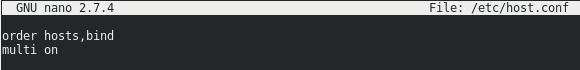
\includegraphics[width=.75 \textwidth]{images/hostconf}
		\caption{Archivo de configuración /etc/host.conf.}
		\label{image:hostconf}
\end{figure}
\FloatBarrier

Así mismo, se cambió el hostname del servidor a \textbf{server1} en el archivo \textbf{/etc/hostname} se agregó una resolución de nombre de dominio al archivo \textbf{/etc/hosts} para indicar que el servidor local es el host y dominio server1.redes3.local:

\FloatBarrier
\begin{figure}[htbp!]
		\centering
			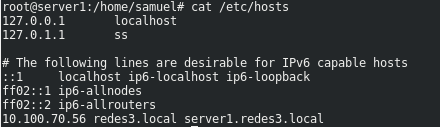
\includegraphics[width=.75 \textwidth]{images/hosts}
		\caption{Archivo de resolución de nombres de dominio.}
		\label{image:hosts}
\end{figure}
\FloatBarrier

Este último paso se debe realizar en cada cliente de la topología que utilice los servicios de correo con la finalidad de que pueda reconocer la dirección IP del dominio.

Una vez configurado la resolución de nombre de dominio y el nombre de host se procede a instalar \textbf{Posfix}. Para ello se utiliza el comando:

\texttt{apt-get install postfix}

Durante la instalación se solicitará ingresar el tipo de configuración general de correo (\textit{General type of mail configuration}). Para lo cual se eligió \textbf{Internet Site}.
De igual forma se solicitará el nombre de sistema de correo en el cual se establece el nombre de host más el nombre de dominio configurado anteriormente: \textbf{server1.redes3.local}.

El siguiente paso es editar la configuración de Postfix desde su archivo \textbf{/etc/postfix/main.cf}. Esta configuración se puede ver reflejada con el comando:

\texttt{postconf -n}

La configuración final se puede observar en la figura \ref{image:postconf}

\FloatBarrier
\begin{figure}[htbp!]
		\centering
			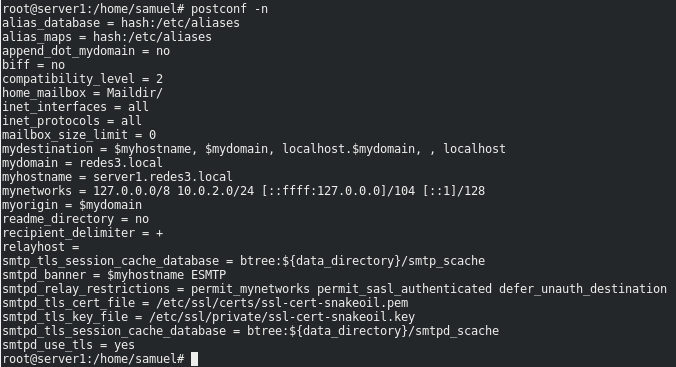
\includegraphics[width=.75 \textwidth]{images/postconf}
		\caption{Configuración final de Postfix.}
		\label{image:postconf}
\end{figure}
\FloatBarrier

El paso siguiente es instalar Dovecot como servidor IMAP. Para ello se utiliza el siguiente comando:

\texttt{apt install dovecot-core dovecot-imapd}

Una vez instalado deberemos editar algunos de los archivos de configuración. El primero es el archivo \textbf{/etc/dovecot/dovecot.conf} en el cual se debe descomentar la línea:

\texttt{listen = *, ::}

El segundo archivo a editar es \textbf{/etc/dovecot/conf.d/10-auth.conf} en el cual se deben tener líneas como las siguientes:

\texttt{disable\_plaintext\_auth = no}

\texttt{auth\_mechanisms = plain login}

El tercer archivo a editar es \textbf{ /etc/dovecot/conf.d/10-mail.conf} en la siguiente línea:

\texttt{mail\_location = maildir:~/Maildir}

Y el último archivo a editar es \textbf{/etc/dovecot/conf.d/10-master.conf} en el bloque de smpt-auth:\\

\texttt{
\# Postfix smtp-auth \\
  	unix\_listener /var/spool/postfix/private/auth \{\\
  	mode = 0666\\
  	user = postfix\\
  	group = postfix\\
 	\}}
 	
Reiniciamos Postfix y Dovecot:

\texttt{service postfix restart}
\texttt{service dovecot restart}

El último paso es la instalación de Rainloop Webmail como cliente de correo electrónico a través de HTTP. Para ello se instala un servidor apache y las dependencias necesarias para utilizar PHP. Para ello, usamos el siguiente comando:

\texttt{apt install apache2 php7.0 libapache2-mod-php7.0 php7.0-curl php7.0-xml}

Eliminamos el archivo índice del Apache y descargamos Webmail:\\
\texttt{\# cd /var/www/html/}\\
\texttt{\# rm index.html}\\
\texttt{\# curl -sL https://repository.rainloop.net/installer.php | php}

Finalizada la instalación procedemos a ingresar al navegador web en la dirección \textbf{http://localhost/?admin} e ingresamos con las credenciales: \textbf{User: admin} y \textbf{Password: 12345} como se muestra en la figura \ref{image:webmail}.

\FloatBarrier
\begin{figure}[htbp!]
		\centering
			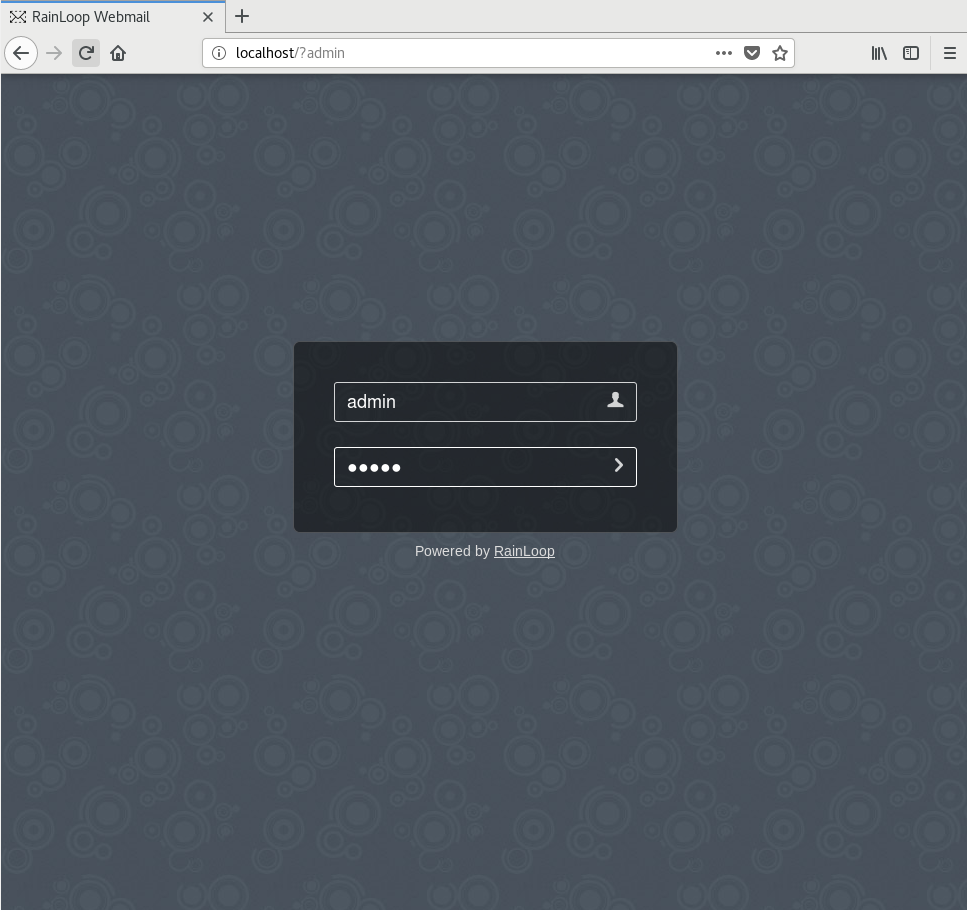
\includegraphics[width=.65 \textwidth]{images/webmail}
		\caption{Login de configuración de Webmail.}
		\label{image:webmail}
\end{figure}
\FloatBarrier

Dentro del panel de configuración nos dirigimos a la pestaña \textbf{Domains} en donde se agrega el dominio configurado al inicio. Esto se puede ver en la figura \ref{image:webmaildomain}.

\FloatBarrier
\begin{figure}[htbp!]
		\centering
			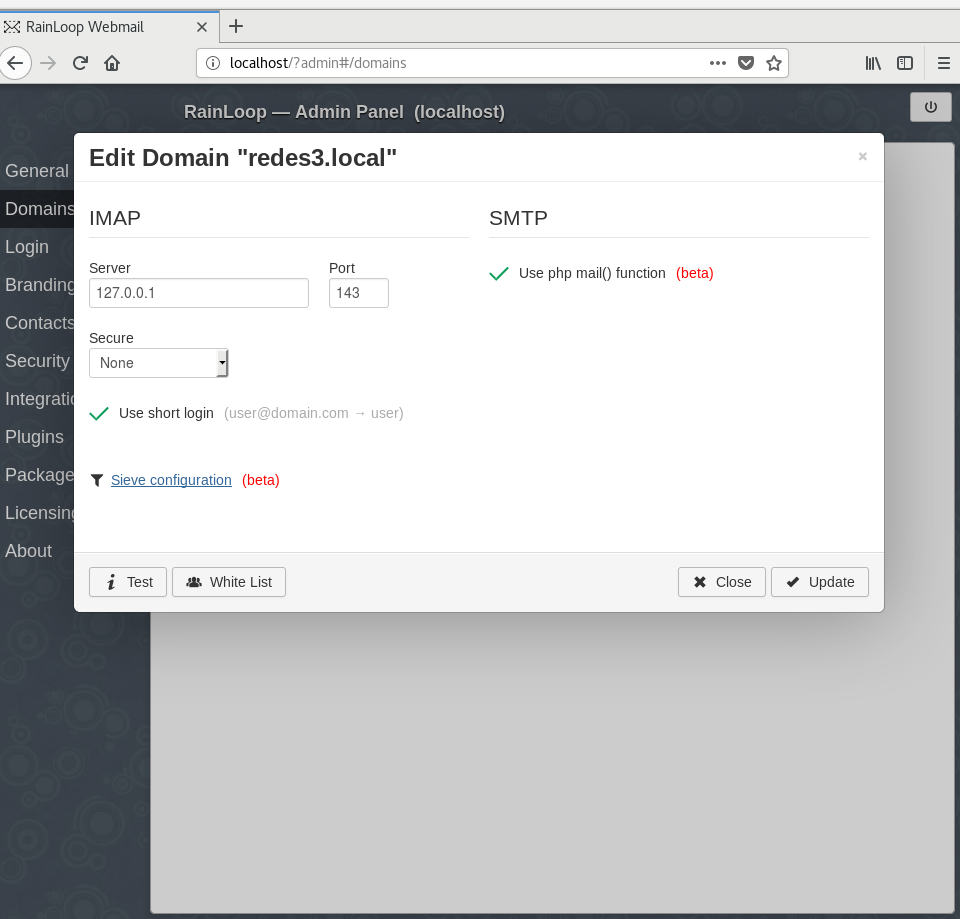
\includegraphics[width=.65 \textwidth]{images/webmaildomain}
		\caption{Configuración de dominio.}
		\label{image:webmaildomain}
\end{figure}
\FloatBarrier

Finalmente, para crear un nuevo usuario en el servidor de correo (SNMP + IMAP) es necesario crear al usuario UNIX. Sin embargo, antes se debe definir una variable global que indique el directorio de almacenamiento de los correos para cada usuario. Para realizar esto se utilizan los siguientes comandos:

\texttt{echo `export MAIL=\$HOME/Maildir' >{}>  /etc/profile}\\
\texttt{useradd -m samuel}\\
\texttt{passwd samuel}

\FloatBarrier
\begin{figure}[htbp!]
		\centering
			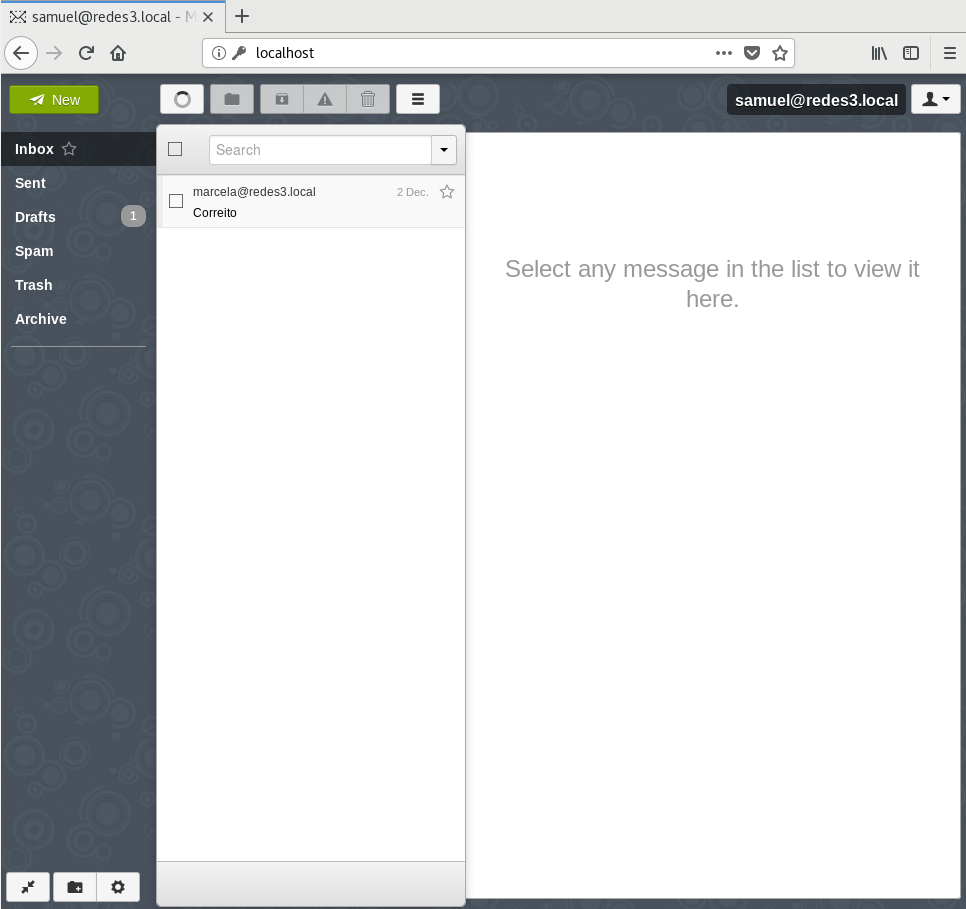
\includegraphics[width=.65 \textwidth]{images/mail}
		\caption{Bandeja de entrada.}
		\label{image:mail}
\end{figure}
\FloatBarrier

\subsection{Sensor SMTP}
El sensor SMTP realiza mediciones de tiempo de respuesta tanto del servidor SMTP como del servidor IMAP. Para ello, se toma el tiempo (EPOCH) antes de realizar una solicitud SMTP, es decir, tiempo inicial. Después, se envía un correo de prueba a un usuario predefinido. Una vez que se terminó de ejecutar la función de solicitud de envío se vuelve a tomar el tiempo. Este tiempo será el tiempo de respuesta del servidor SMTP, puesto que el servidor SMTP ya terminó su tarea de enviar el correo al servidor IMAP. No obstante, para obtener el tiempo de respuesta del servidor IMAP se obtiene el nombre del último archivo modificado en la bandeja de entrada del usuario de prueba. Por defecto, Dovecot almacena los correos en el sistema de archivos concatenando en el nombre el tiempo (EPOCH) en el que fue recibido. Es por ello, que este valor se considera el tiempo de respuesta del servidor IMAP.

El proceso se muestra a detalle en la función \textbf{sensor\_correo()} de la figura \ref{image:sensorcorreo}. Dicha función es parte del programa \textbf{cliente.py} escrito en Python que contiene la funcionalidad de todos los sensores solicitados en esta práctica.

\FloatBarrier
\begin{figure}[htbp!]
		\centering
			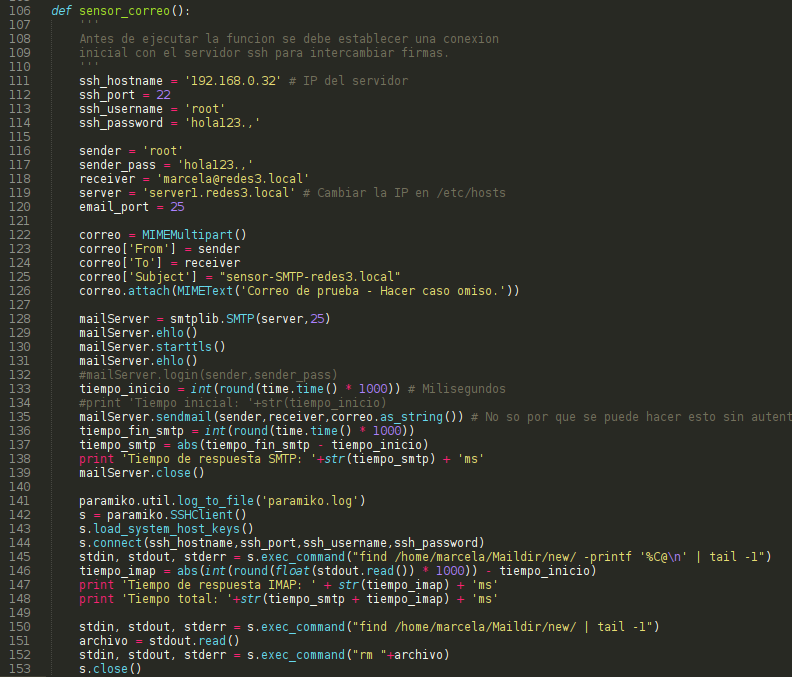
\includegraphics[width=.65 \textwidth]{images/sensorcorreo}
		\caption{Código en Python del sensor de correo.}
		\label{image:sensorcorreo}
\end{figure}
\FloatBarrier

De la línea 122 a la línea 131 se realiza la preparación del correo de prueba. En a línea 133 se toma el tiempo inicial y posteriormente, en la línea 135 se realiza la solicitud de envío SMTP. Una vez que termina, en la línea 136 se vuelve a tomar el tiempo que indica la respuesta SMTP. A partir de la línea 141 a la línea 153 se realiza una conexión mediante SSH para obtener el tiempo EPOCH del nombre del último archivo modificado en la bandeja de entrada del usuario de prueba. Finalmente, utilizando SSH se elimina el correo de prueba.

\subsubsection{Funcionamiento}
Inciamos corriendo el programa \textbf{cliente.py} de la siguiente manera:\\
\texttt{python cliente.py}\\
Se despliega el menú de opciones y elegimos la opción 1 que corresponde al sensor SMTP. Con ello, el sensor realizará todas las operaciones antes mencionadas y mostrará en pantalla los tiempos obtenidos como se puede observar en la figura \ref{image:sensorcorreofunc}

\FloatBarrier
\begin{figure}[htbp!]
		\centering
			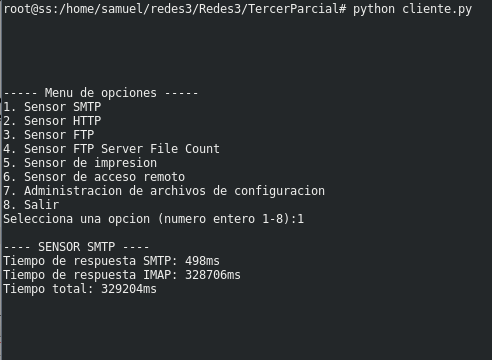
\includegraphics[width=.65 \textwidth]{images/sensorcorreofunc}
		\caption{Funcionamiento del sensor de correo.}
		\label{image:sensorcorreofunc}
\end{figure}
\FloatBarrier